\documentclass[12pt,letterpaper,titlepage]{article}

\usepackage{fontspec}
\defaultfontfeatures{Mapping=tex-text}
\usepackage{xunicode}
\usepackage{xltxtra}
\usepackage{amsmath}
\usepackage{pdfpages}
\usepackage{amsfonts}
\usepackage{amssymb}
\setcounter{secnumdepth}{0}
\usepackage{nameref}
\usepackage{enumitem}
\usepackage{environ}
\usepackage{pgfplots}

\setmainfont{Times New Roman}
\showboxdepth=\maxdimen
\showboxbreadth=\maxdimen


\usepackage{paracol}
\usepackage{wrapfig}
\globalcounter{table}
\globalcounter{figure}
\usepackage{graphicx}
\usepackage[left=1in,right=1in,top=1in,bottom=1in]{geometry}
\graphicspath{{img/}}

\author{Jacob Abel}
\title{	Homework 1
	\\\large ECE3544 CRN:82989
}

\setlength{\parskip}{0.25em}

\begin{document}
\maketitle
\begin{raggedright}
\begin{paracol}{2}
\paragraph{Problem 1: }
Using 2's complement arithmetic, add the following decimal numbers, showing all work. i.e. perform $17+19$. Use the smallest number of bits possible to represent each number and the sum without overflow. 
\begin{align*}
17+19 	&= 010001 + 010011
\\		&= 010010 + 010010
\\		&= 010100 + 010000
\\		&= 100100
\\		&= 36
\end{align*}
\paragraph{Problem 2: }
For the addition in problem 1, use one less bit to represent the numbers and show how the overflow can be detected.
\begin{align*}
17+19 	&= 10001 + 10011
\\		&= 10010 + 10010
\\		&= 10100 + 10000
\\		&= 00100
\\		&= 4
\end{align*}
Overflow can be detected during addition for unsigned integers when the most significant bit changes from $1$ to $0$.
\switchcolumn
\paragraph{Problem 3: }
Using the same guidelines as for problem 1, subtract decimal $87$ from $37$, i.e. perform $37-87$.
\begin{align*}
37-87 	&= 00100101 - 01010111
\\		&= 00100101 + 10101001
\\		&= 00100110 + 10101000
\\		&= 01001110 + 10000000
\\		&= 11001110
\\		&= -00110010
\\		&= -50
\end{align*}
\paragraph{Problem 4: }
Give the hexadecimal representation of the answer to problem 3.
\begin{align*}
37-87 	&= -50
\\		&= 1100 1110
\\		&= CE_{16}
\end{align*}
\end{paracol} 
\paragraph{Problem 5: }
Write the truth table and Boolean function implemented by the CMOS gate below.
\begin{center}
\begin{paracol}{3}
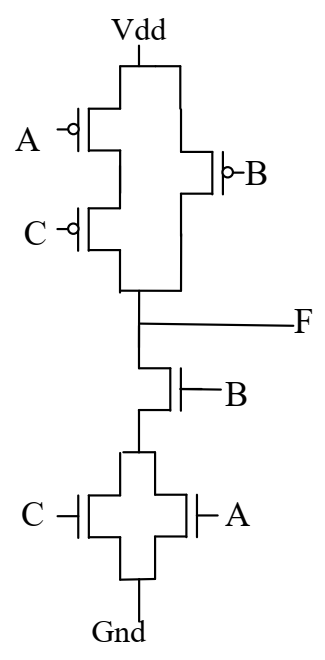
\includegraphics[width=\textwidth, height=15\baselineskip, keepaspectratio=true]{hw1q5}
\switchcolumn
{\renewcommand{\arraystretch}{0.9}
\begin{tabular}{|ccc|c|}
\hline
   A & B & C & F 
\\\hline
   0 & 0 & 0 & 1
\\ 0 & 0 & 1 & 1
\\ 0 & 0 & 0 & 1
\\ 0 & 0 & 1 & 1
\\ 0 & 1 & 0 & 1
\\ 0 & 1 & 1 & 0
\\ 0 & 1 & 0 & 1
\\ 0 & 1 & 1 & 0
\\ 1 & 0 & 0 & 1
\\ 1 & 0 & 1 & 1
\\ 1 & 0 & 0 & 1
\\ 1 & 0 & 1 & 1
\\ 1 & 1 & 0 & 0
\\ 1 & 1 & 1 & 0
\\ 1 & 1 & 0 & 0
\\ 1 & 1 & 1 & 0
\\\hline
\end{tabular}}
\switchcolumn
$F = \overline{B \cdot (A + C)}$

\end{paracol}
\end{center}
\clearpage
\paragraph{Problem 6: }
Draw transistor schematics of a CMOS gate for each of the following Boolean functions:
\begin{paracol}{2}
\begin{center}
$F=\overline{(W+Z)\cdot(Y+X)}$

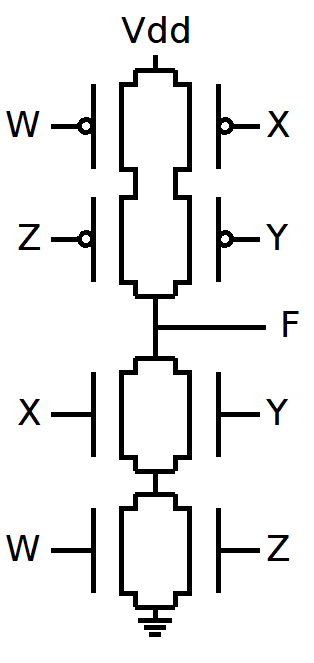
\includegraphics[width=\textwidth, height=17\baselineskip, keepaspectratio=true]{hw1q6a}
\end{center}

\switchcolumn
\begin{center}
$G=\overline{(B+C+D)\cdot A}$

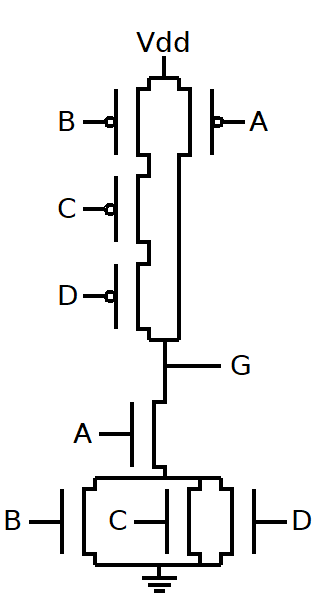
\includegraphics[width=\textwidth, height=17\baselineskip, keepaspectratio=true]{hw1q6b}
\end{center}
\end{paracol}

\paragraph{Problem 7: }
Which would you expect to have a bigger effect on the power consumed by a CMOS circuit, a $5\%$ increase in the power supply voltage ($V_{dd}$) or a $10\%$ increase in total capacitance? Briefly explain your answer.

$P=CV^2f\implies\Delta P = \Delta C\times (\Delta V)^2\times \Delta f$

$\Delta C = 110\%$ and $(\Delta V)^2 = (105\%)^2 = 110.25\%$

The voltage increase will have a slightly larger effect.

\end{raggedright}
\end{document}
